\documentclass{standalone}
\usepackage{xcolor}
\definecolor{thmColor}{rgb}{0.95,0.05,0.05}%
\usepackage{tikz}

\begin{document}
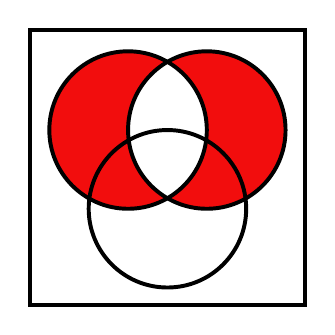
\begin{tikzpicture}[line width=0.5mm,fill=thmColor]
\scope
\clip (-1.75,-1.8) -- (-1.75,1.7) -- (1.75,1.7) -- (1.75,-1.8) -- cycle
      (-0.5,0.425) circle (1);
\fill (0.5,0.425) circle (1);
\endscope
\scope
\clip (-1.75,-1.8) -- (-1.75,1.7) -- (1.75,1.7) -- (1.75,-1.8) -- cycle
      (0.5,0.425) circle (1);
\fill (-0.5,0.425) circle (1);
\endscope
%
\draw (-0.5,0.425) circle (1);
\draw (0,-0.575) circle (1);
\draw (0.5,0.425) circle (1);
\draw (-1.75,-1.8) -- (-1.75,1.7) -- (1.75,1.7) -- (1.75,-1.8) -- cycle;
\end{tikzpicture}
\end{document}
